%Jennifer Pan, August 2011

\documentclass[10.5pt,letter]{article}
	% basic article document class
	% use percent signs to make comments to yourself -- they will not show up.

\usepackage{amsmath}
\usepackage{tikz}
\usepackage{amssymb}
	% packages that allow mathematical formatting
\usepackage{mathtools}
\usepackage{graphicx}
	% package that allows you to include graphics

\usepackage{setspace}
	% package that allows you to change spacing

\onehalfspacing
	% text become 1.5 spaced

\usepackage{fullpage}

\graphicspath{ {images/} }
	% package that specifies normal margins
	

\begin{document}
	% line of code telling latex that your document is beginning


\title{CS124 Programming Assignment 3}

\author{HUID 51248651}

\date{04/21/2017}
	% Note: when you omit this command, the current date is automatically included
 
\maketitle 
	% tells latex to follow your header (e.g., title, author) commands.
	
\paragraph{Warm-up Exercise} Suppose that the integers $a_1, ... a_n$ in $A$ sum to $b$. Then thinking about the problem as partitioning the set into two separate sets and looking at the residue as the difference of their sums, we have that it would be ideal to split $A$ into two sets $S_1$ and $S_2$, such that the elements in $S_1$ and $S_2$ both sum to $b/2$, which would yield a residue of $0$, which is clearly the lower bound on residue. If $b$ is odd, then we would want $S_1$ to have elements summing to $\lfloor b/2 \rfloor$, with $S_2$ then clearly summing to $\lceil b/2\rceil$, giving a residue of $1$. Thus we want to see if there is a way to create a subset of $A$ such that its elements sum to $\lfloor b/2 \rfloor$. If this is not possible, then we want to try to create one that sums to $\lfloor b/2 \rfloor -1$, then $\lfloor b/2\rfloor -2$ and so on and so forth until it is possible to create such a set. It is eventually possible to, since the empty set sums to $0$. Thus, let $C(\alpha, A)$ be a subset of $A$ whose members sum to $\alpha$, and if there is no such set, $C(\alpha, A) = null$. Then our recurrence relation is that (let $A'$ be the element from $A$ with highest index, given that $A$ initially equals to $a_1, ... a_n$, so $A'$ of $a_1, a_2, a_4 = a_4$. Define $A'$ as having value $val(A')$). If $C(\alpha-val(A'), A\backslash A') \neq null$, then $C(\alpha, A) = A' \cup C(\alpha-val(A'), A\backslash A')$. Else if $C(\alpha, A \backslash A') \neq null$, then $C(\alpha, A) = C(\alpha, A \backslash A') $, Else, $C(\alpha, A) = null$. The first two options represent the choice to either include or not include $A'$ in our resultant set, and the third is when neither two options succeed. Recursive base cases: $C(0, B) = \emptyset$, $C(a, B) = null$ if $a < 0$, and $C(a, \emptyset) = null$ if $a \neq 0$.

 Our algorithm then runs as follows: Let $i =0$, let $result = null$. Then while $(result = C(\lfloor b/2\rfloor - i, A)) = null,$ $i = i + 1$. We then convert $result$ to a sequence of negative and positive numbers in our returned sequence $S$ having $s_j = 1$ if $a_j \in result$, else $s_j = -1$. Then by our dynamic programming paradigm, every time we compute $C(\beta, B)$, for some set $B$ and value $\beta$, we store the resultant set in an array, so we only calculate each set once and can there after access each set in $O(1)$ time. \\ \\
Proof of Correctness: Our recursive relation is correct, because either our resultant set contains the element $A'$, or it doesn't, and if neither option yields a set with the correct sum, then such a set is impossible to create. Our base cases our trivially correct, as if we are trying to construct a set which sums to $0$, the empty set works, and it is impossible to construct a set with negative sum, since our supposition is that the elements given to us are nonnegative. Lastly, it is impossible to construct a set with non-zero sum from the empty set. Then our ideal partition is one which gives one set that sums to $\lfloor b/2 \rfloor$, necessarily making the other sum to $\lceil b/2 \rceil$. Then if this is not possible, we reduce our target sum by one, and continue until we find a value which works. This is our optimal set.
Runtime Analysis: We calculate each set $C(\beta, B)$ once, then can access it in $O(1)$ time since we store it in an array. $\beta$ can take values ranging from $0$ to $\lfloor b/2\rfloor$. Then our $B$ set is constructed from $A$ by systematically lopping off the highest index element left in its parent set. Thus if $A= a_1, ... a_n$, then $B$ can be any member of the set of sets of the form $\{ \{ a_1, .. a_j\} \}$, $j \in [1, n]$, or the empty set. There are $n+1$ such sets, so we have that $B$ can take $n+1$ different values. Thus there are $O(nb)$ values which compute and store in our array, so our memory usage is $O(nb)$. Then since each computation of $C(\beta, B)$ is $O(1)$ given that we have already computed the other recursive values, we have that the runtime is also $O(nb)$. $\blacksquare$


\paragraph{Karmarkar-Karp in O(nlogn) steps} Assuming that the values in $A$ are small enough that arithmetic operations take one step, we can first put the elements of $A$ into binary max heap, $Q$. Constructing it using max-heapify is an $O(nlogn)$ operation. Then, we continuously pop the top two elements off of $Q$, call these elements $a_1, a_2$, where $a_1$ is the first element popped, so $a_1 \ge a_2$. We then insert $a_1 - a_2$ into $Q$, an $O(log n)$ operation. Else, if there is only one element left in the heap, ie it is empty after popping off $a_1$, we return $a_1$ as the Karmarkar-Karp calculated residue. \\
Runtime: This algorithm runs in $O(nlogn)$ steps, because it builds the heap once in $O(n log n)$ time, and then performs less than $n$ insertions, each with cost $O(logn)$, thus the total runtime of all insertions is $O(nlogn)$. Then all other operations run in constant time, so we have that our overall algorithm is $O(nlogn)$, as desired.  \\
Proof of correctness: Karmarkar-Karp works by removing the the two greatest elements from the list $A$, then replacing them with $0$ and their difference. It repeats this until there is only one non-zero element left, then returns it as an obtainable residue. Clearly, my algorithm performs the same series of operations, the only difference being that it doesn't add the $0$ back into the heap. This doesn't effect the result, because the largest two elements chosen while never contain a zero, and if it does then the algorithm should terminate (ie one non-zero element left), which is what my algorithm does. 

\paragraph{Discussion of programming Karmakar-Karp} I implemented my program in Java. I used longs to store my numbers, since the standard int overflows on $10^12$. I initially programmed a MergeSort, and then performed Karmarkar-Karp off of a list $A$ by mergesorting it, replacing the largest two entries with zero and their difference, and then mergesorting again, and repeating until only one nonzero entry was left, then returned that value. This meant that my Karmarkar-Karp was $O(n^2logn)$, since I performed $n$ mergesorts. While this was fine for 1 list of 100 numbers, when attempting to run 100 instances of the problem, and iterate at least 25000 times on each algorithm, the pre-partitioning representation of the problem proved prohibitively slow, since it was running Karmarkar-Karp 25000 times on each instant,  times 3 for the 3 different methods. In order to solve this problem, I improved my Karmarkar-Karp by first mergesorting the list, and then subsequently performing a linear pass of the list when inserting $|a_j-a_i|$ into it. It was possible since the rest of the list was already sorted, I just needed to stick in a lone value in the correct place. In this manner, I reduced my Karmarkar-Karp $O(nlogn + n^2) = O(n^2)$, since I was performing one mergesort then $n-1$ linear insertions. While this was better, my the 25000 iterations still took a non-trivial amount of time, so I decided to go for it an implemented an array-based binary heap in Java. This reduced my Karmarkar-Karp to $O(nlogn)$, since from an array $A$ of numbers I constructed a maximum heap of them in $O(nlogn)$ time, and then while the size of the heap was greater than $1$, I popped off the top two elements and then inserted their difference. Each pop is $O(1)$, and each insertion was $O(logn)$. I performed at most $n$ such insertions, so that component was also $O(nlogn)$. Furthermore, I constructed my heap class such that length is a tracked property, so retrieving it is $O(1)$. Thus the overall algorithm was $O(nlogn)$. 

\paragraph{Discussion of random number generation} I used Java's built in Random class to generate my random longs for the graphing portion of this problem set. Since Random can only generate integers, and $10^12$ is out of the range of integer, for each random long I independently generated two random integers $a_1$, $a_2$ uniformly distributed between $0$ and $1E6- 1$, inclusive. Then I defined my random long in $[1, 1E12]$ as being $a_1*1E6 + a_2 + 1$ In this way, the digit at each position in my resultant number is randomly generated, while only making two calls to random. I add one to my resultant long since otherwise my interval of random longs would be $[0, 1E12 -1]$. 

\pagebreak

\paragraph{Table of Data}  I've included raw data on my first 32 instances of the problem, where each time is given in milliseconds, as computed by the Java system. Having a $1$ in the name indicates that the problem was represented in the standard way of a solution $S$ containing a $1$ or $-1$ at each position. A $2$ in the the name indicates that the problem was represented via prepartitioning. I did not include the runtime of the lone Karmarkar-Karp iteration, since they were all registered as $0$ milliseconds by Java. I used 50,000 iterations.

\begin{figure}[h!]
 \centering 
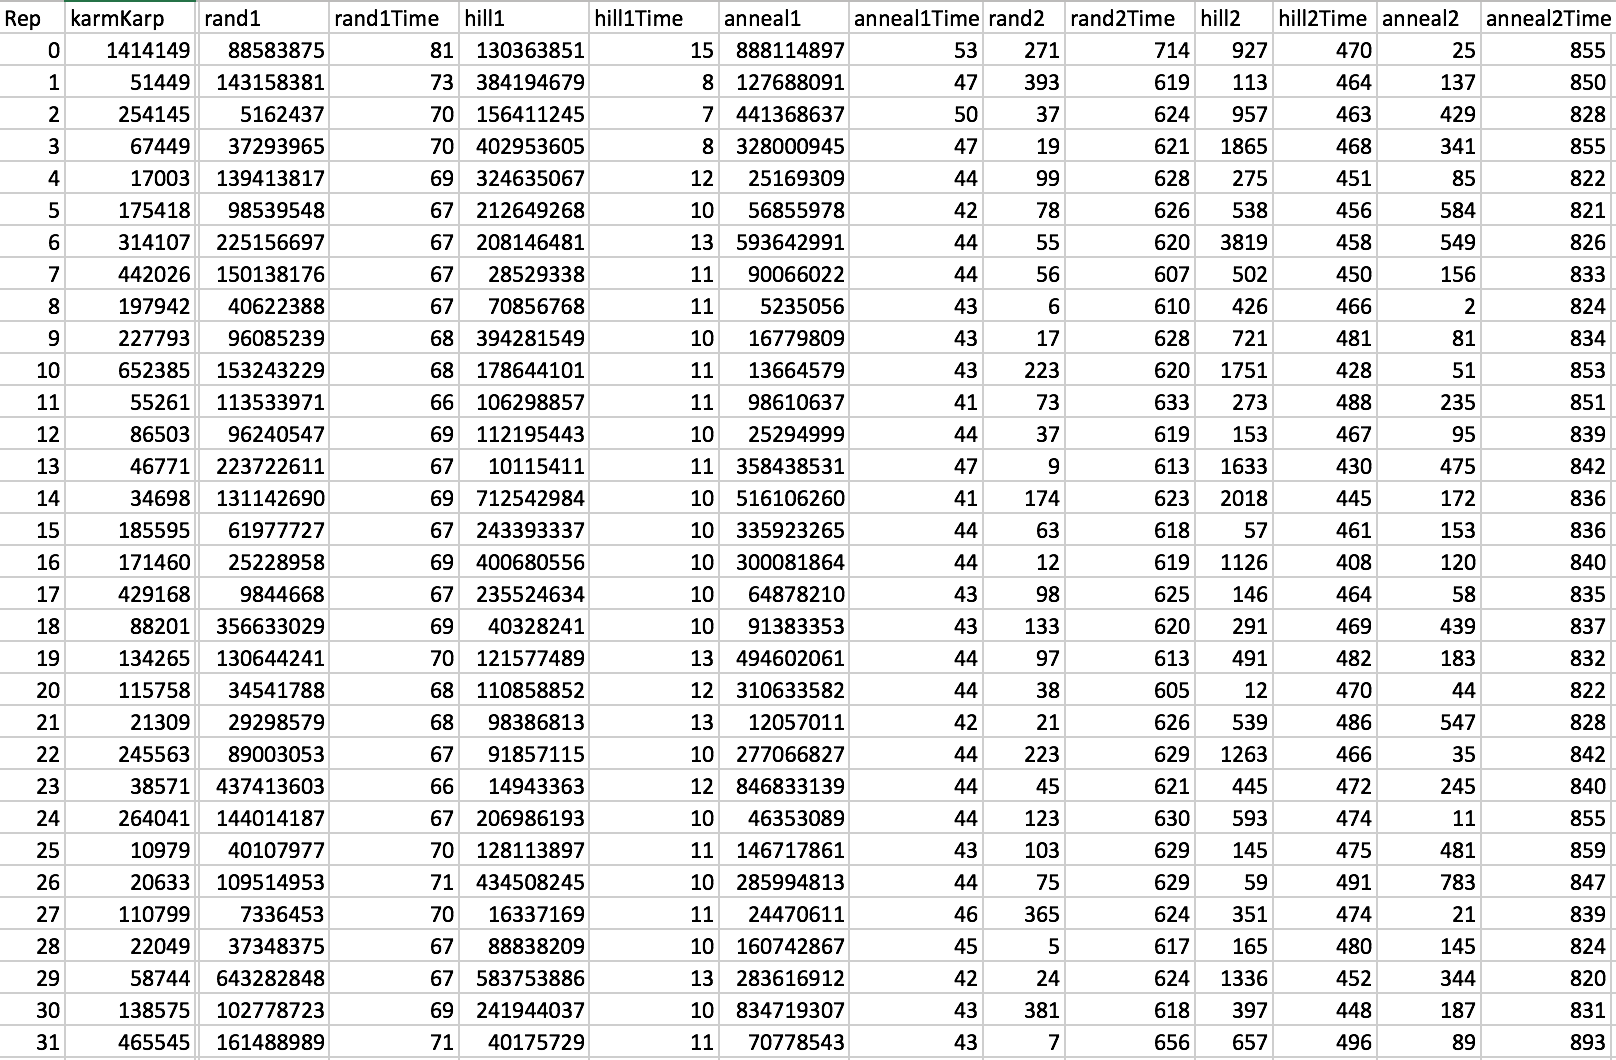
\includegraphics[scale=0.66]{firstThird}
\end{figure}


Then over 100 instances of the problem, where each instance was an array of 100 numbers uniformly distributed between $[1, 1E12]$, I had the following average values: \\


{\setlength{\tabcolsep}{11pt}
\begin{tabular} {|c | c | c | c | c | c | } \hline  
Karmarkar-Karp = 189,048.84 & Repeated Random (1) =130,225,432 & Rep Rand Runtime (1) = 69.27 \\ \hline
Hill-Climb (1) = 258,803,414 & Hill-Climb Runtime (1) = 10.72 & Sim Anneal (1) = 236,895,158 \\ \hline
 Sim Anneal Runtime (1) = 43.82  & Repeated Random (2) = 87.94 & Rep Rand Runtime (2) = 629.58 \\ \hline
 Hill-Climb (2) = 711.5 & Hill-Climb Runtime (2) = 470.58 & Sim Anneal (2) = 214.86 \\ \hline 
 & Sim Anneal (2) Runtime = 841.1 \\ \hline

\end{tabular}} \\ \\

Note that I ran all of these with 50,000 iterations. \\

From this data, we observe that Hill-Climbing was for both representations the worst algorithm. On representation $1$, it's calculated residue was two times that of repeated random searching. I believe this was because hill-climbing is incredibly dependent on the initial random solution, and if that solution is poor, then the overall algorithm is rather sunk. On the second representation, Hill-Climbing was $\approx 5$ times worse than either repeat random or simulated annealing. This is a larger difference, and it is so large because Karmarkar-Karp is ultimately used to calculate the residue on a pre-partitioning representation. Since Karmarkar-Karp computes a "pretty good" residue off of a given set, this means that the second representation compounds the inefficiency of hill-climbing due to its dependence on the initial solution, Furthermore, neighbors in the pre-partitioning representation are more similar than those in the standard representation when it comes time to calculate residue, since we are not deciding which set each element is in, but simply which elements must be grouped together. \\
On the standard representation, we have that simulated annealing and hill climbing yielded roughly the same average value, which make sense as both are roughly equivalently dependent on the starting random solution. Simulated annealing did yield a slightly better value, which makes sense as it has access to a larger universe of neighbors about the initial solution, do to the probabilistic manner in which it sets $S=S'$ regardless. Also, we always return the best found partition, by virtue of the inclusion of $S''$. \\
On pre-partition representation, we get that simulated annealing is roughly twice as good as hill climbing. This is a larger factor than in the standard representation, which I believe makes sense as performing Karmarkar-Karp in order to calculate the residue yields an increased probability that the randomness of assigning $S=S'$ introduced in annealing will ultimately yield a significantly lower result. It makes sense that repeated random is the best of all three on pre-partitioning, as in this way we are no longer dependent on the arbitrary merit of our initial random solution. \\

In general, the pre-partitioning representations yielded order of magnitudes better results across all three algorithms. I believe that this is sensical as performing Karmarkar-Karp, which is necessary to compute pre-partitioned residues, yields a "very good" residue on the set, so for each random solution our pre-partition residue is far lower than our standard representation residue. \\ \\
Discussion of the runtimes: I did not include the runtime of the individual Karmarkar-Karp in my data table, as it was clocked at $0$ milliseconds by Java. We have on the standard representation that hill climb was faster than annealing was faster than repeated random, which makes sense as for repeated random we had to calculate a large number of random numbers, while with simulated annealing we add in the additional complexity of computing $T(iter)$ as well as making additional residue computations. \\
All three algorithms were far faster on the standard representation than the were on the pre-partitioning representation.This makes sense, as each time we calculated residue on the pre-partitioning representation it was necessary to call Karmarkar-Karp which, though being an $O(nlogn)$ function, contributes a large amount to the runtime over 50,000 iterations. \\ \\



\paragraph{Using Karmarkar-Karp as starting point for randomized algorithms} Given the Karmarkar-Karp implicitly generates a partition of the set when computing an achievable residue, we could use the partition $P$ generated by Karmarkar-Karp on a set $A$ an the starting random solution $S$ in our repeated random, hill climbing, and simulated annealing algorithms.\\
Doings so would not significantly effect the way that repeated random worked, since on each iteration it generates a completely new solution. It would probably make the algorithm yield slightly better results, especially for small number of iterations, since we are guaranteed a solution at least as good as that yielded by Karmarkar-Karp. \\
For the Hill-Climbing algorithm, it would yield better results since at each iteration we are computing a neighbor of the previous iteration. Thus since our starting solution is already "pretty good" since it comes from Karmarkar-Karp, the algorithm will be randomly exploring a sequence of neighbors of a solution that is already good, so the neighbors of it will be better than if $S$ were randomly selected. \\
For the Simulated annealing algorithm, the logic as to why the Hill-Climbing algorithm is better when running Karmarkar-Karp first largely holds, with the addition that since we with set$S=S'$ even when $S'$ has greater residue with some probability, we will have access to a larger neighborhood of solutions about our starting solution. I hypothesize that this will mean that the improvement over standard annealing wont be as dramatic, since this algorithm is therefore in general not quite as dependent on its starting solution, as it more freely traverses the universe of neighbors.



\end{document}
	% line of code telling latex that your document is ending. If you leave this out, you'll get an error
